\documentclass[12pt,oneside]{book}


\usepackage[utf8]{inputenc}
\usepackage[T1]{fontenc}
\usepackage{graphicx}
\usepackage{amsmath}
\usepackage{amssymb}
\usepackage{multicol}
\usepackage{natbib}

\usepackage{hyperref}

\usepackage[a4paper,width=175mm,top=20mm,bottom=20mm,bindingoffset=6mm]{geometry}
\usepackage{fancyhdr}
\pagestyle{fancy}

\begin{document}
\title{Multi-agent Maintenance Scheduling: \\ The Making of a Science}
\author{Christian Brunbjerg Jespersen}
\date{\today}
\maketitle

\tableofcontents

\begin{multicols}{2}
\chapter{Introduction}
Maintenance scheduling is in its nature a multi actor process. Many stakeholders have to coordinate in both time and space to allow for an
efficient and effective execution. This thesis will propose a generalized multi-agent scheduling system and it will argue that for the field of
maintenance scheduling to more forward similar approaches will have to be adopted. Other approaches may be very different but they will share many 
of the aspects. 

This Ph.D. will present a generalized dynamic multi-model approach to maintenance scheduling which will be model after a practical maintenace handbook \cite{palmer_maintenance_2019}.
This book written by the experienced practitioner Richard D. Palmer will be a guiding light throughout the thesis, so it serves as the main source and validation, 
or maybe invalidation is a better word, as we explore the academic maintenance scheduling literture and also, and more importantly, it will also be the source 
which above all else will us us through the perilous process of create a generalize model setup for maintenance scheduling.



\section{The General Maintenance Scheduling Process}
This section will provide an overview of the maintenance scheduling process in the most abstracted way possible. It will be important to understand this setup
throughly as most industries that perform maintanance of a considerable scale follow this process. Many industries are of course unique and deviate
from general framework in specific work but the fundamentals are usually quite similar. 

\begin{figure}[H]
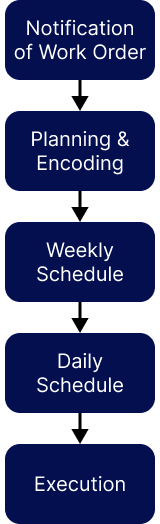
\includegraphics[width=1.0\textwidth]{figures/top-level-schedule-overview.png}
\label{top-level-schedule-overview.png}
\end{figure}





\chapter{Modelling the Generalized Setup}
To model the maintenace process in its entirety we will need tool that are powerful enough to describe the system. The system will be described in accordance 
with the \ref{top-level-schedule-overview.png} \cite{palmer_maintenance_2019}.

The maintenance scheduling problem is NP-hard and real-time optimal solutions will never be a feasible approach unless we use a multi-model setup where each model enriches the 
overall solution in the way that it is most capable of. 

\input{tex/literature_review}
\newcommand{\MessageQueue}{Q}
\newcommand{\Solution}{X}
\newcommand{\ProblemInstance}{P}
\newcommand{\SharedSolution}{S}

\begin{algorithm}[H]
\caption{Actor-based Large Neighborhood Search} 
\begin{algorithmic}[1]
\State \textbf{Input} $\MessageQueue$    = message queue
\State \textbf{Input} $\ProblemInstance$ = problem instance
\State \textbf{Input} $\Solution$        = initial schedule
\State \textbf{Input} $\SharedSolution$  = shared solution
% \State $\Solution^b = \Solution$
\Repeat \label{alg:actor-based-large-neighborhood-search:main-optimization-loop}
	\State $\Solution^t = clone(\Solution)$ \label{alg:actor-based-large-neighborhood-search:clone-solution}
	\While{$\MessageQueue.has\_message()$} \label{alg:actor-based-large-neighborhood-search:message-loop}
        % \State $m = queue.pop()$
        % \State $m.destruct(\Solution^b)$
		\State $\ProblemInstance.update(\SharedSolution, m)$
        \State $\Solution^t.destruct(\SharedSolution, m)$
    \EndWhile
	
    \State $\Solution^t.repair(\SharedSolution)$ \label{alg:actor-based-large-neighborhood-search:repair}

    \If{accept($\Solution^t, \Solution$)} \label{alg:actor-based-large-neighborhood-search:accept}                       
        \State $\Solution.update(\Solution^t)$
    \EndIf                                         

    \If{$c(\Solution^t) < c(\Solution)$} \label{alg:actor-based-large-neighborhood-search:better-solution}                             
        \State $\Solution.update(\Solution^t)$
		\State $\SharedSolution.atomic\_pointer\_swap(\Solution)$
    \EndIf                                           
	\State $\MessageQueue.push(m)$ \label{alg:actor-based-large-neighborhood-search:schedule-message}
\Until
\end{algorithmic}
\label{alg:actor-based-large-neighborhood-search}
\end{algorithm}




possible sections
* All Stochasticity will be handled by user interaction. 
* In maintenance scheduling, data is assumed to be correct. Yes that must be the prevailing idea here.

\input{tex/verification-study}
\section{Discussion}
\label{sec:4-discussion}
Maintenance scheduling efficiently solves a complex scheduling problem by the use of multiple actors. Through the use of actors the 
process handles uncertainty that is difficult to reason about, using models with different levels of aggregation where each actors understands
how to exploit his model. As uncertainties manifest themselves the actors/models handle the uncertainty through 
communication. To further understand the implications of the approach the discussion will be divided into three sections: 1. actors and 
integration; 2. continuous optimization allows asynchronous optimization; 3. future research.

\subsection{Actors \& Integration}
Often in operation research the failure to reliably solve industry problems are not due to the problems being computationally intractable 
but more a practical problem of connecting data streams so that the solution approach is connected to dynamic data source of the company
and then connecting the solution approach(s) to the relevant stakeholder (actors) through a relevant interface. The actor-based approach 
proposed in this paper makes integration easier by naturally encapsulation a model with a reliable interface. To better understand the 
novel properties of this consider the extension of figure 

\ref{fig:simple-maintenance-process}

as shown in figure \ref{fig:integrated:maintenance-process}.


\begin{figure}[H]
\centering
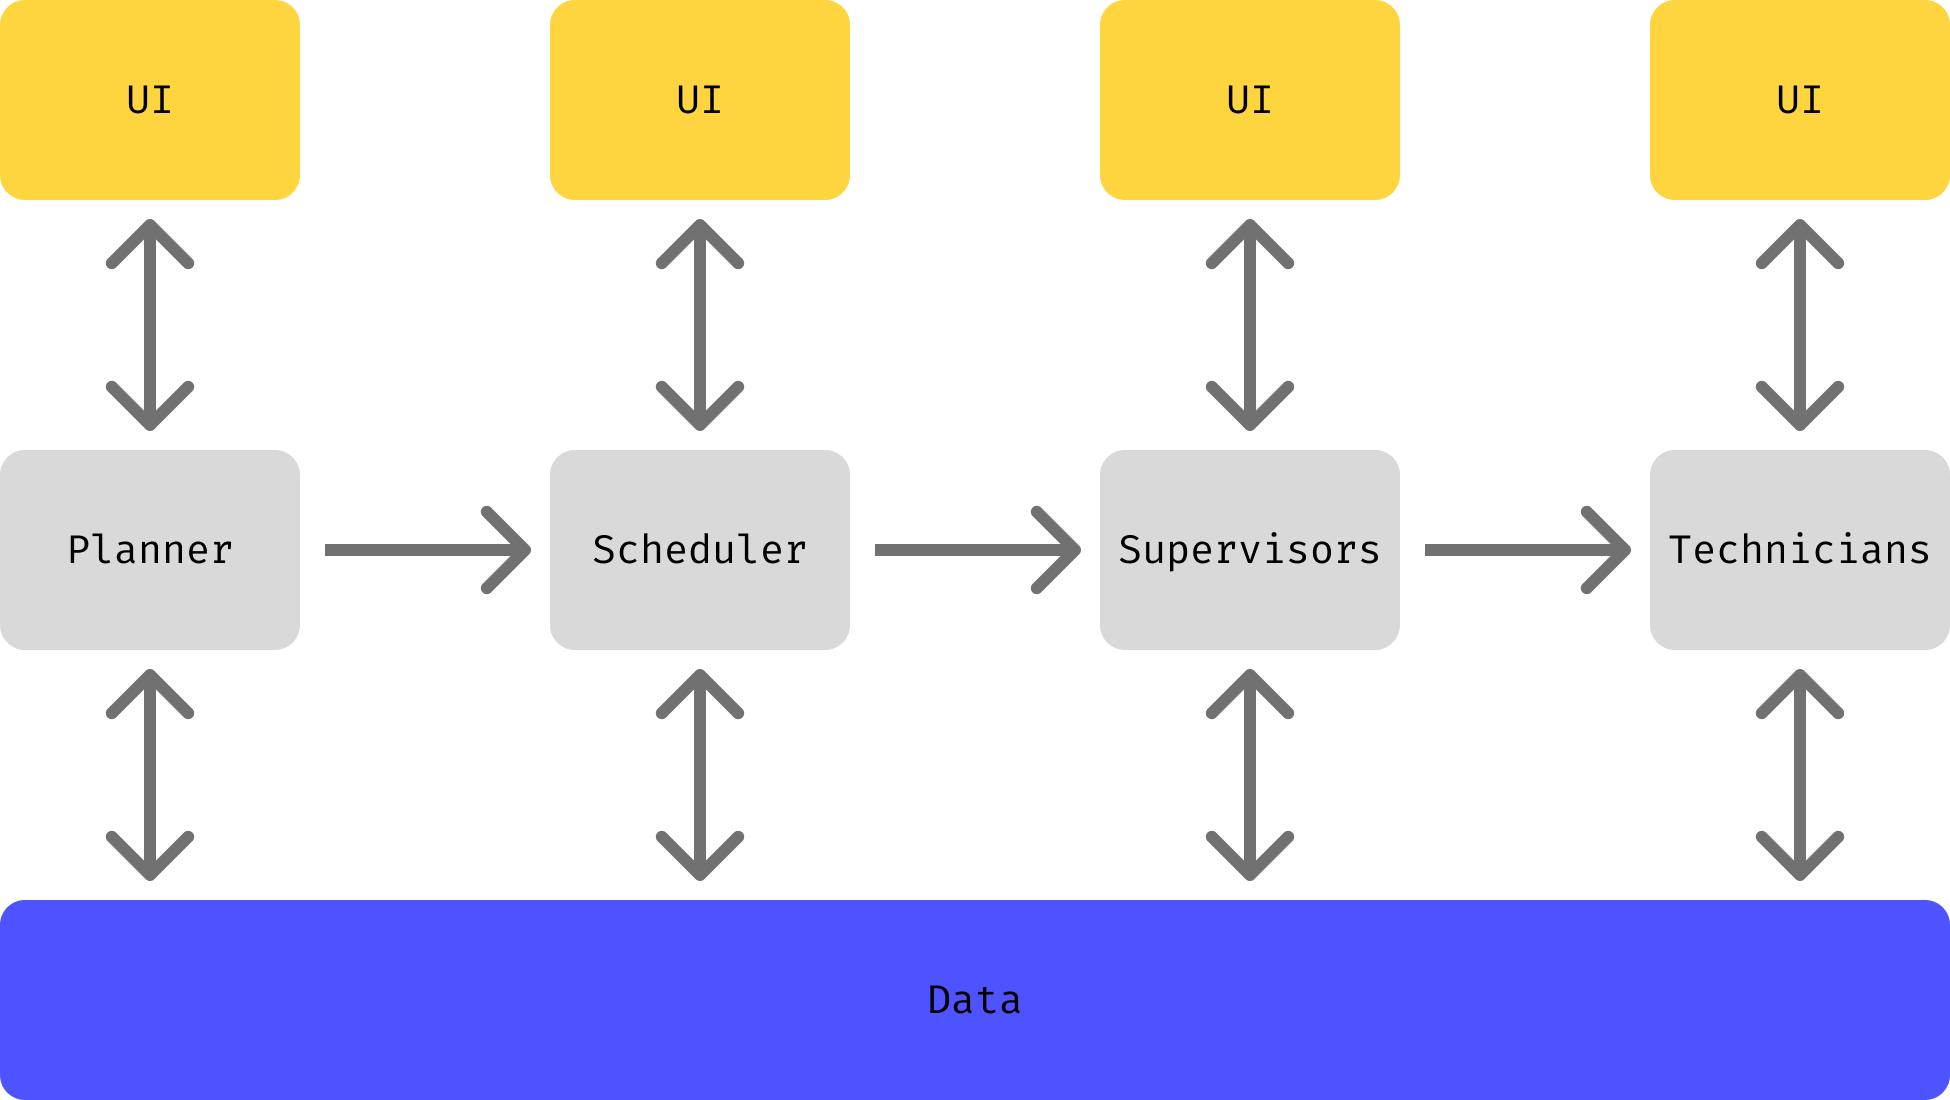
\includegraphics[width=1.0\textwidth]{figures/Scheduling Process Integrated.png}
\label{fig:integrated:maintenance-process}
\caption{Overview of the scheduling process when modelled as actors. When LNS is encapsulated 
is an actor it becomes possible to optimize parts of a large process individually instead of 
optimizing the scheduling problem globally from a single model inplementation.}
\end{figure}


\subsection{Continuous Optimization}
With actor-based metaheuristics it becomes simple to extend a metaheuristic to run
indefinitely with it being able to optimize based on the latest best 
available information. This may seem like a minor detail as you could argue that you should only ever optimize the schedule when there is 
an explicit need for it, but consider the case when you start adding more than two actor to a scheduling system, then there arises a need
to coordinate people in time as each will have to run their optimizer on after another.

\input{tex/conclusion}
\end{multicols}
\appendix
\input{appendices/appendixA}


\bibliographystyle{plainnat}
\bibliography{bib/references}

\end{document}
